\documentclass[conference]{IEEEtran}
\IEEEoverridecommandlockouts

\usepackage{cite}
\usepackage{amsmath,amssymb,amsfonts}
\usepackage{algorithmic}
\usepackage{graphicx}
\usepackage{textcomp}
\usepackage{xcolor}
\usepackage[a4paper, total={184mm,239mm}]{geometry}
\def\BibTeX{{\rm B\kern-.05em{\sc i\kern-.025em b}\kern-.08em
    T\kern-.1667em\lower.7ex\hbox{E}\kern-.125emX}}

\usepackage{listings}
\usepackage{booktabs}
\usepackage{multirow}
\usepackage[normalem]{ulem}
\useunder{\uline}{\ul}{}
\usepackage{url}
\usepackage{fancyvrb}

\lstdefinestyle{Scalastyle}{
    language=scala,
    aboveskip=3mm,
    belowskip=3mm,
    showstringspaces=false,
    columns=flexible,
    basicstyle={\small\ttfamily},
    numberstyle=\tiny\color{gray},
    keywordstyle=\color{blue},
    commentstyle=\color{dkgreen},
    stringstyle=\color{mauve},
    breaklines=true,
    breakatwhitespace=true,
    tabsize=2,
    numbers=left,
    xleftmargin=2em,
    frame=single,
    framexleftmargin=1.5em,
    captionpos=b
}

\definecolor{mGreen}{rgb}{0,0.6,0}
\definecolor{mGray}{rgb}{0.5,0.5,0.5}
\definecolor{mPurple}{rgb}{0.58,0,0.82}
\definecolor{backgroundColour}{rgb}{0.95,0.95,0.92}

\lstdefinestyle{Cstyle}{
    language=C,
    aboveskip=3mm,
    belowskip=3mm,
    showstringspaces=false,
    columns=flexible,
    basicstyle={\small\ttfamily},
    numberstyle=\tiny\color{gray},
    keywordstyle=\color{blue},
    commentstyle=\color{mGreen},
    stringstyle=\color{mPurple},
    breaklines=true,
    breakatwhitespace=true,
    tabsize=2,
    numbers=left,
    xleftmargin=2em,
    frame=single,
    framexleftmargin=1.5em,
    captionpos=b
}

\begin{document}

\title{Paper title}

\author{
    \IEEEauthorblockN{1st author}
    \IEEEauthorblockA{
        \textit{dept. name of organization (of Aff.)} \\
        \textit{name of organization (of Aff.)}\\
        City, Country \\
        email address or ORCID
    }
    \and
    \IEEEauthorblockN{2nd author}
    \IEEEauthorblockA{
        \textit{dept. name of organization (of Aff.)} \\
        \textit{name of organization (of Aff.)}\\
        City, Country \\
        email address or ORCID
    }
    \and
    \IEEEauthorblockN{3rd author}
    \IEEEauthorblockA{
        \textit{dept. name of organization (of Aff.)} \\
        \textit{name of organization (of Aff.)}\\
        City, Country \\
        email address or ORCID
    }
}


\maketitle

\begin{abstract}
Abstract
\end{abstract}

\begin{IEEEkeywords}
    3-5 keywords
\end{IEEEkeywords}

%We want to lower costs with energy efficiency as well
\section{Introduction}
U interaktivnim simulacijama i računalnim igrama, ključno je brzo i precizno detektirati sudare izmedu objekata zbog funkcionalnosti te interaktivnosti. Što su scenariji u videoigrama složeniji, to su algoritmi za detekciju sudara zahtjevniji u smislu računalnih resursa. Ovaj zahtjev može rezultirati smanjenjem performansi, što utječe na korisničko iskustvo. Navedeni problem postaje posebno izražen kod izvodenja u stvarnom vremenu, gdje je brza reakcija presudna.\\
Ideja ovog projekta je razviti model paralelizacije u C++ za algoritam detekcije sudara koji efikasno koristi višedretvenost na procesoru. Simulacije će biti vizualizirane korištenjem OpenGL, programskim sučeljem za razvoj grafičkih aplikacija. Navedeni alat omogućuje programerima renderiranje 2D i 3D scena. Cilj projekta je optimizirati performanse algoritma za detekciju sudara kroz raspodjelu zadataka na više jezgri procesora, koristeći podržane mehanizme višedretvenosti.\\
Testiranje paralelizacije algoritma provoditi će se na simuliranih scenarijima padajućih loptica različitih ulaznih parametara. Mjerit će se brzina izvodenja algoritma te korištenje računalnih resursa kako bi pratili efikasnost paralelizacije.
\section{Background}
\subsection{Theoretical concepts}
Integracija Verletova algoritma je matematička metoda koja se često koristi za izračunavanje putanja kretanja čestica u računalnoj grafici. Algoritam integrira Newtonove jednadžbe gibanja.
U jednadžbi Verletove integracije  \( \mathbf{x}_n \) predstavlja poziciju na koraku n,  \( \mathbf{a}_n \) predstavlja akceleraciju na koraku n.
\[
\mathbf{x}_{n+1} = 2\mathbf{x}_n - \mathbf{x}_{n-1} + \mathbf{a}_n \Delta t^2
\]
Pojednostavljivanjem jednadžbe dobivamo sljedeće:
\[
\mathbf{x}_{n+1} = \mathbf{x}_n + - \mathbf{v}_{n}\Delta t 
\]
Za implementaciju simulacije sudara loptica potrebno je minimizirati preklapanje izmedu loptica. Vrijednost preklapanja dvije loptice računamo oduzimanjem udaljenosti izmedu središta loptica od zbroja njihovih radijusa.

\begin{figure}
    \centering
    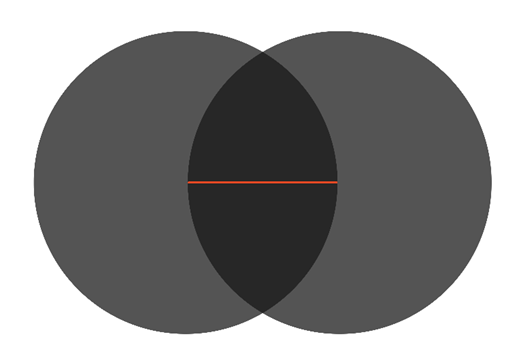
\includegraphics[width=0.5\linewidth]{image.png}
    \caption{Preklapanje loptica}
    \label{fig:enter-label}
\end{figure}

 Medutim, za samu simulaciju potrebno je računati preklapanja svih loptica unutar simulacije kako bi mogli otkloniti sva preklapanja loptica. Sljedeće je moguće napraviti naivnim pristupom u kojem iteriramo prvo po svakoj loptici, a zatim po ostalim lopticama te pomičemo loptice ako se preklapaju. Naivni pristup je ispravan u kontekstu otklanjanja preklapanja, ali je vrlo spor zbog složenosti izvodenja. Broj provjera preklapanja jednak je broju loptica na kvadrat. \\ 
Optimalan pristup problemu preklapanja loptica je podjela prostora na kvadratne dijelove. Odredujemo da je duljina stranice kvadrata ista kao i dijametar kuglice. Zatim svakom kvadratnom dijelu prostora pridodjeljujemo loptice čije središte se nalazi u njemu. Ovim korakom svaki dio dobiva listu loptica. Nakon toga iteriramo kroz sve kvadratne dijelove i računamo udaljenosti izmedu trenutnog i susjednog kvadratnog dijela prostora. U iteracije nisu uključeni “vanjski” dijelovi.


\subsection{Related work}


\section{Main}

\subsection{Subsection}



\subsection{Subsection}


\subsubsection{Subsubsection}


\subsubsection{Subsubsection}


\subsubsection{Subsubsection}



\section{Evaluation}
\subsection{Methodology}


\subsection{Results}

\subsection{Discussion}



\section{Conclusion}
Future work

Citation examples:

Journal paper \cite{Koeplinger2018}

Conference paper \cite{Siefke2022}

Link \cite{Gapuino}


\bibliographystyle{IEEEtran}
\bibliography{refs}

\end{document}
